\documentclass[12pt]{article}

\usepackage{amsmath,amssymb}
\usepackage{geometry}
\usepackage{graphicx}
\usepackage{array}
\usepackage{enumitem}
\usepackage{listings}
\usepackage{xcolor}
\usepackage{titlesec}

\geometry{margin=1in}

%  BLUE COLOR 
\definecolor{mainblue}{RGB}{0,0,180}

% SECTION FORMATTING
\titleformat{\section}
  {\color{mainblue}\normalfont\Large\bfseries}
  {}{0em}{}

\titleformat{\subsection}
  {\color{mainblue}\normalfont\large\bfseries}
  {}{0em}{}

\titlespacing*{\section}{0pt}{1.5em}{0.8em}
\titlespacing*{\subsection}{0pt}{1em}{0.5em}

% ======= CODE STYLE=====
\lstset{
    basicstyle=\ttfamily\small,
    frame=single,
    breaklines=true
}

\begin{document}

% ======= HEADER =====
\begin{minipage}{0.3\textwidth}
    
\includegraphics[width=0.8\textwidth]{logo.png}
\end{minipage}
\hfill
\begin{minipage}{0.6\textwidth}
\begin{flushright}
\textbf{Name:} Chinmayi VV\\
\textbf{Batch:} COMETFWC041\\
\textbf{Assignment:} GATE Question 11\\
\textbf{Date:} 16 Feb 2026
\end{flushright}
\end{minipage}

\vspace{1.2cm}

% ======== MAIN TITLE====
\begin{center}
\fontsize{24}{28}\selectfont
\textbf{\color{mainblue}GATE Question 11 Analysis and Hardware Verification}
\end{center}

\vspace{1.2cm}

% ========= QUESTION ========
\section*{Question 11}

Match the logic gates in Column A with their equivalents in Column B.

\begin{center}
\begin{tabular}{|c|c|}
\hline
\textbf{Column-A} & \textbf{Column-B} \\
\hline
1. AND Gate & P. XOR Gate \\
2. OR Gate  & Q. XNOR Gate \\
3. NOT Gate & R. NAND Gate \\
\hline
\end{tabular}
\end{center}

\vspace{1cm}

% ====== QUESTION ANALYSIS ======
\section*{Question Analysis}

\begin{itemize}
\item AND gate gives output 1 only when both inputs are 1.
\item OR gate gives output 1 when at least one input is 1.
\item NOT gate inverts the input.
\item NAND is complement of AND.
\item NOR is complement of OR.
\item XOR gives output 1 when inputs are different.
\item XNOR gives output 1 when inputs are equal.
\end{itemize}

Thus logical equivalences are verified using Boolean algebra and truth tables.

\vspace{1cm}

% ====== BOOLEAN EXPRESSIONS====
\section*{Boolean Expressions}

\begin{itemize}
\item AND Gate: $Y = A \cdot B$
\item OR Gate: $Y = A + B$
\item NOT Gate: $Y = \overline{A}$
\item NAND Gate: $Y = \overline{A \cdot B}$
\item NOR Gate: $Y = \overline{A + B}$
\item XOR Gate: $Y = A \oplus B$
\item XNOR Gate: $Y = \overline{A \oplus B}$
\end{itemize}

\vspace{1cm}

% ====== TRUTH TABLES ===
\section*{Truth Tables}

% AND
\subsection*{AND Gate}
\begin{center}
\begin{tabular}{|c|c|c|}
\hline
A & B & Output \\
\hline
0 & 0 & 0 \\
0 & 1 & 0 \\
1 & 0 & 0 \\
1 & 1 & 1 \\
\hline
\end{tabular}
\end{center}

% OR
\subsection*{OR Gate}
\begin{center}
\begin{tabular}{|c|c|c|}
\hline
A & B & Output \\
\hline
0 & 0 & 0 \\
0 & 1 & 1 \\
1 & 0 & 1 \\
1 & 1 & 1 \\
\hline
\end{tabular}
\end{center}

% NOT
\subsection*{NOT Gate}
\begin{center}
\begin{tabular}{|c|c|}
\hline
A & Output \\
\hline
0 & 1 \\
1 & 0 \\
\hline
\end{tabular}
\end{center}

% NAND
\subsection*{NAND Gate}
\begin{center}
\begin{tabular}{|c|c|c|}
\hline
A & B & Output \\
\hline
0 & 0 & 1 \\
0 & 1 & 1 \\
1 & 0 & 1 \\
1 & 1 & 0 \\
\hline
\end{tabular}
\end{center}

% NOR
\subsection*{NOR Gate}
\begin{center}
\begin{tabular}{|c|c|c|}
\hline
A & B & Output \\
\hline
0 & 0 & 1 \\
0 & 1 & 0 \\
1 & 0 & 0 \\
1 & 1 & 0 \\
\hline
\end{tabular}
\end{center}

% XOR
\subsection*{XOR Gate}
\begin{center}
\begin{tabular}{|c|c|c|}
\hline
A & B & Output \\
\hline
0 & 0 & 0 \\
0 & 1 & 1 \\
1 & 0 & 1 \\
1 & 1 & 0 \\
\hline
\end{tabular}
\end{center}

% XNOR
\subsection*{XNOR Gate}
\begin{center}
\begin{tabular}{|c|c|c|}
\hline
A & B & Output \\
\hline
0 & 0 & 1 \\
0 & 1 & 0 \\
1 & 0 & 0 \\
1 & 1 & 1 \\
\hline
\end{tabular}
\end{center}

\vspace{1cm}

% ====== ARDUINO CODE =======
\section*{Arduino Code for Seven Segment Display}

\begin{lstlisting}[language=C++]
#include <Arduino.h>

void sevenseg(int a,int b,int c,int d,int e,int f,int g)
{
  digitalWrite(2, a);
  digitalWrite(3, b);
  digitalWrite(4, c);
  digitalWrite(5, d);
  digitalWrite(6, e);
  digitalWrite(7, f);
  digitalWrite(8, g);
}

void setup()
{
  for(int i=2; i<=8; i++)
  {
    pinMode(i, OUTPUT);
  }
}

void loop()
{
  sevenseg(1,0,0,1,1,1,1);
  delay(1000);

  sevenseg(0,0,1,0,0,1,0);
  delay(1000);

  sevenseg(0,0,0,0,1,1,0);
  delay(1000);
}
\end{lstlisting}

\vspace{1cm}

% ======== CODE UPLOADING ========
\section*{Code Uploading Steps}

\begin{enumerate}
\item Create PlatformIO project.
\item Write code in main.cpp.
\item Run pio run to generate hex file.
\item Copy hex file to ArduinoDroid.
\item Connect Arduino using OTG.
\item Upload using Upload Precompiled option.
\item Verify seven segment output.
\end{enumerate}

\vspace{1cm}

% === HARDWARE OUTPUT ===
\section*{Hardware Output Verification}

\begin{center}
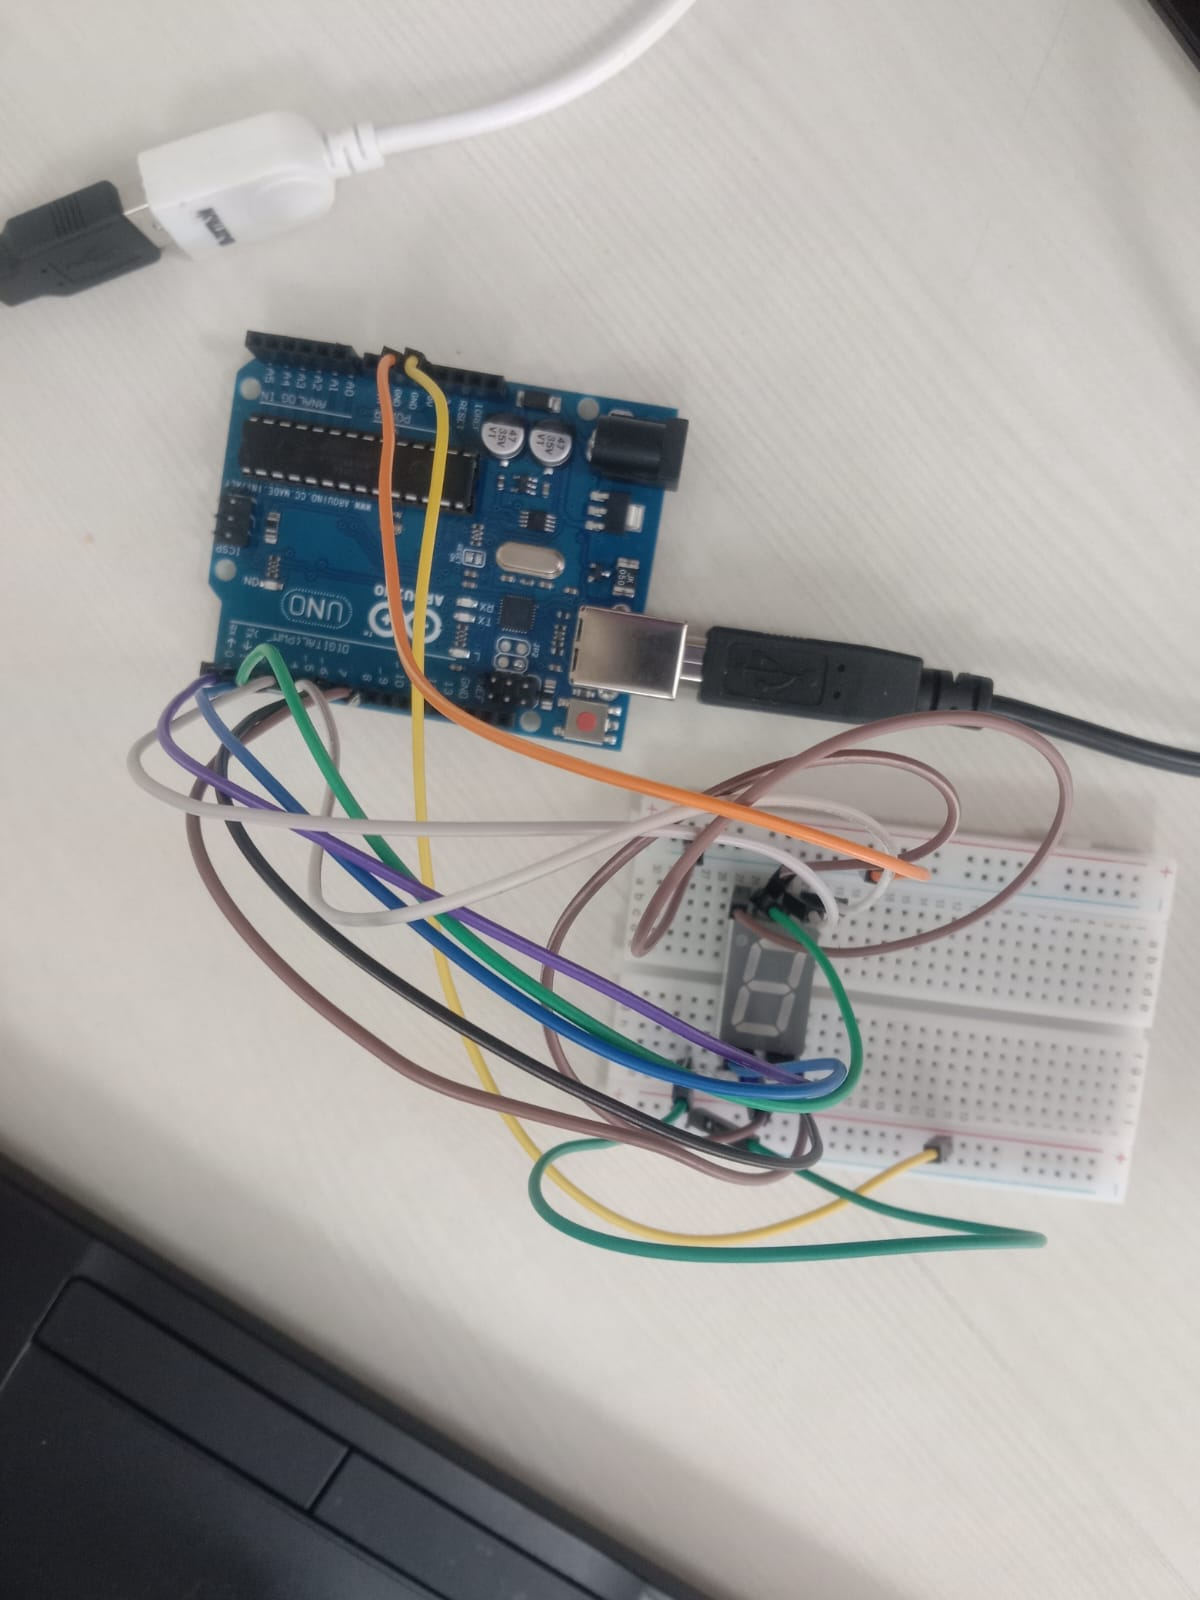
\includegraphics[width=0.7\textwidth]{seven_segment_output.png}

\textbf{Figure: Seven Segment Display Output}
\end{center}

\vspace{1cm}

% ===== CONCLUSION ======
\section*{Conclusion}

All fundamental logic gates and derived gates were analyzed using Boolean algebra and verified through complete truth tables.  
The theoretical study was implemented practically using Arduino UNO and a seven segment display.  
The experimental output confirms correctness of digital logic principles.

\end{document}
